\section{Architektur}
Wir beschreiben im Folgenden die Architektur von helios, die derzeit wie in Abbildung ~\ref{fig:hardarchitecture}) konzipiert ist: helios stellt Schnittstellen bereit, die vom Spiel - verstanden als Echtzeit-Datenmodell~\cite[525]{Gre19} - genutzt werden.\\
Das Framework visualisiert den aktuellen Zustand des Spiels und leitet Daten der Eingabeverarbeitung als Steuerkommandos an dieses weiter.\\

\begin{figure}[!h]
    \centering
    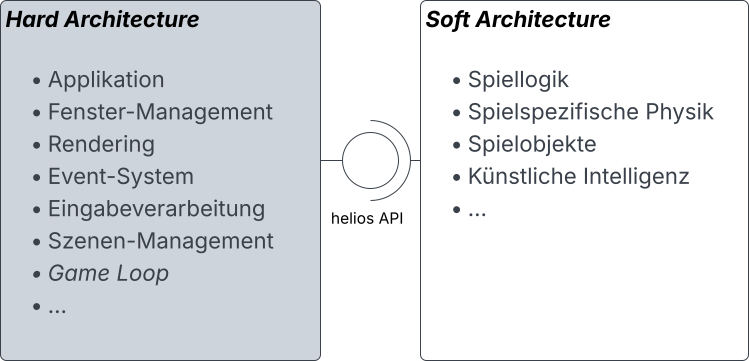
\includegraphics[width=1\columnwidth]{img/hardarchitecture.svg}
    \caption{Aufteilung der Architektur des helios Frameworks in \textit{Hard} und \textit{Soft Architecture} nach \textit{Rollins und Morris}~\cite[612 ff.]{RM04}. Die Ball-/Socket-Notation deutet an, dass helios Schnittstellen zur Verfügung stellt, die ein (beliebiges) Spiel nutzen kann. (Quelle: eigene)}
    \label{fig:hardarchitecture}
\end{figure}

In Abbildung~\ref{fig:package_diagram} ist eine detailliertere Sicht auf die Module und ausgewählter Komponenten dargestellt.
Die Verzeichnisstruktur von helios spiegelt die Gliederung seiner Kernfunktionalitäten wieder.
Im Sinne von \textit{Evans} ist dies entscheidend für die Realisierung einer hohen Kohäsion: Die Verzeichnisnamen kommunizieren die enthaltenen Funktionalitäten~\cite[180 f.]{Eva03}.
Innerhalb der Module findet, wo erforderlich, eine weitere Unterteilung nach Schichten statt (etwa \texttt{controller})\footnote{
im allgemeinen Sprachgebrauch wird diese Strukturierung auch als ``package by feature`` bezeichnet
}.\\


\begin{figure*}[t]
    \centering
    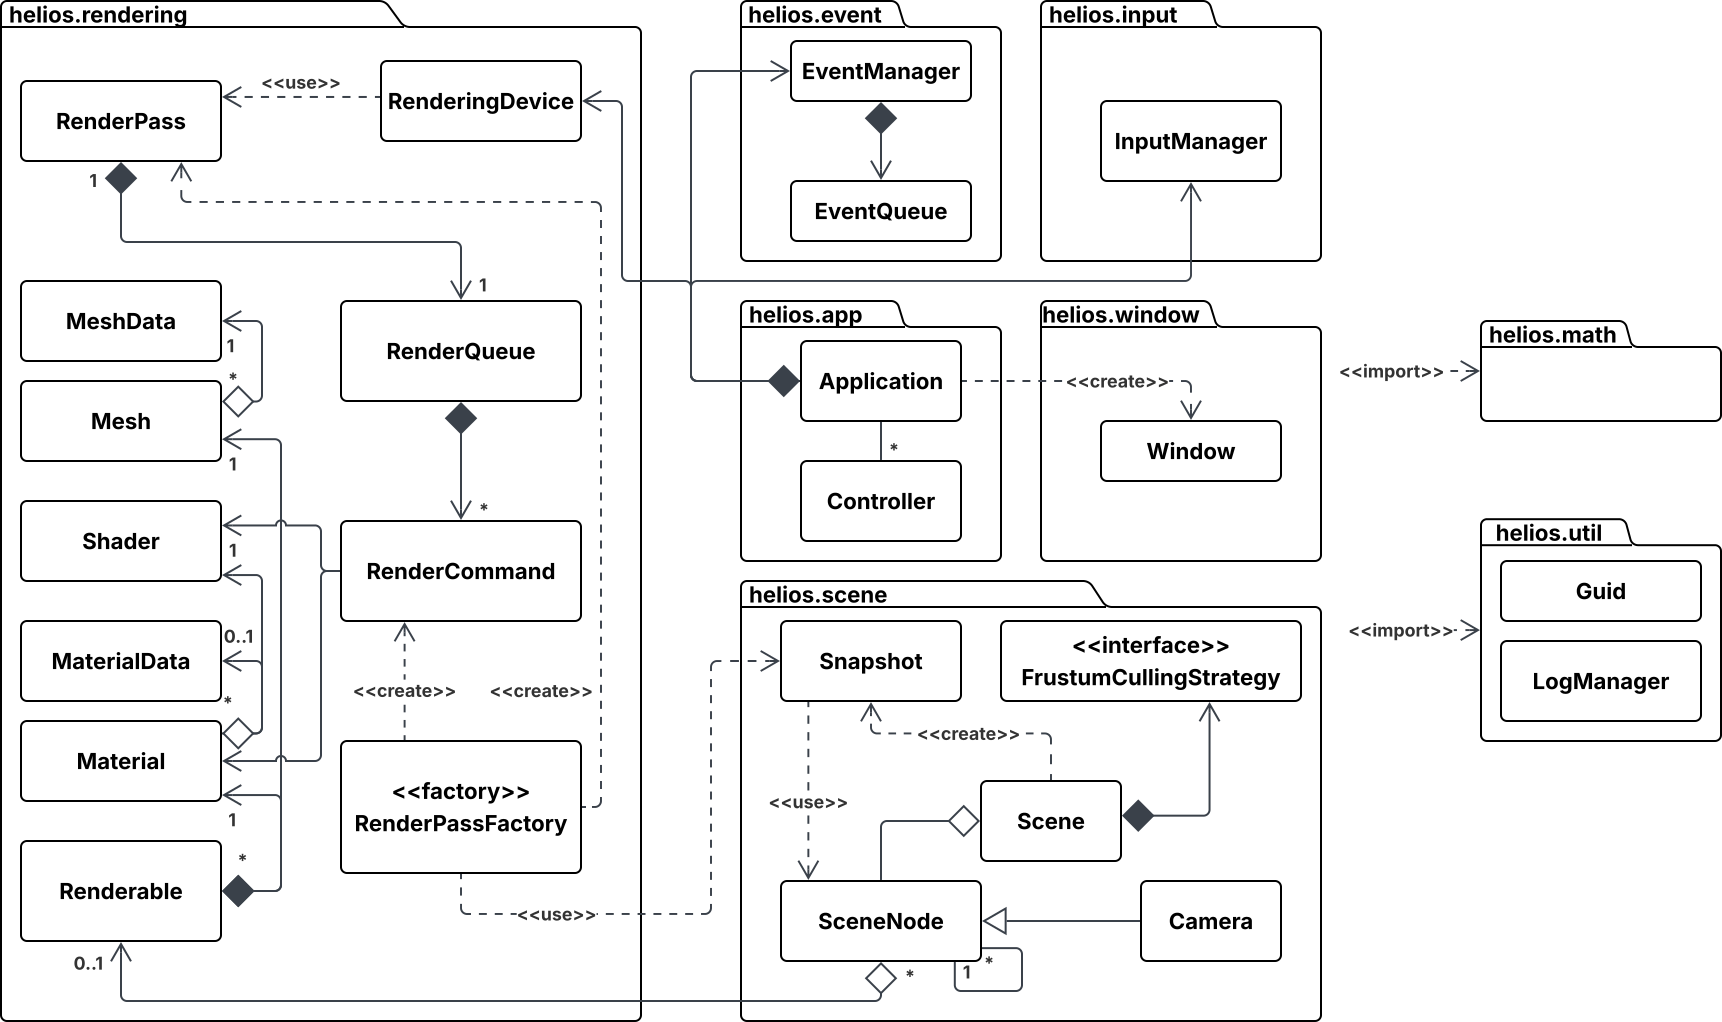
\includegraphics[width=1\textwidth]{img/package_diagram.svg}% \linewidth == Spaltenbreite
    \caption{Aufbau des helios Framework und der Zusammenhang einiger ausgewählter Komponenten. Die Strukturierung der Module orientiert sich an einem ``by Feature, by Layer``-Konzept. (Quelle: eigene)}
    \label{fig:package_diagram}
\end{figure*}


\subsection*{\texttt{app}: Applikationsschicht}
Als zentrale Steuereinheit der Anwendung (also des Spiels) sehen wir eine \texttt{Application}-Klasse vor, die über Event-System, Eingabeverarbeitung und Fenstermanagement verfügt sowie das Rendering-Backend - repräsentiert durch \texttt{RenderDevice} - initialisiert.\\
helios unterstützt an dieser Stelle außerdem dynamisches Hinzufügen von Applikations-Controllern~\cite[379]{Fow03} zur Definition von isolierter, ereignisbasierter Steuerungslogik, bspw. dem Verhalten bei einem Window-Resize\footnote{
Tatsächlich wurden die Applikations-Controller zunächst implementiert, um ``Framebuffer-Resize``-Ereignisse von dem verwendeten Rendering Backend zu abstrahieren.
}.

\subsection*{\texttt{input}: Eingabeverarbeitung}
Die Eingabeverarbeitung orchestriert der \texttt{InputManager}, der exklusiv von der Anwendung verwaltet und von dieser an das derzeit aktive Fenster gebunden wird.\\
Zu Beginn der Game Loop findet ein Polling über die gerade aktiven Eingabeereignisse statt, die nachfolgend über die Schnittstelle des \texttt{InputManager}s abgefragt werden können.
Die Abstraktion der Ereignisse übernimmt hierbei ein \texttt{InputAdapter}, der die durch die TPLs zur Verfügung gestellten Eingabeereignisse abstrahiert.\\
Im weiteren Verlauf der Entwicklung soll eine Factory aus den Eingabeereignissen \texttt{ControlCommand}s erzeugen, die als Eingabeparameter zur Steuerung des Spiels weitergeleitet werden~\cite[21 ff.]{Nys14}.

\subsection*{\texttt{event}: Ereignisverarbeitung}
Ereignisse können über den \texttt{EventManager} in eine \texttt{EventQueue} geschrieben werden (``post``).
Interessierte Entitäten (die ``Beobachter`` bzw. \textit{Observer}) können sich über Callbacks mittels \texttt{subscribe} bei dem EventManager registrieren~\cite[293 ff.]{GHJV94}.
\texttt{EventManager::dispatchAll()} wird zu Beginn der Game Loop aufgerufen und sorgt dann dafür, dass die \texttt{EventQueue} die registrierten Beobachter über vorhandene Ereignisse informiert.

\subsection*{\texttt{window}: Fensterklasse}
Die \texttt{Window}-Klasse stellt Schnittstellen zur Steuerung des Anwendungsfensters bereit, außerdem zur Abfrage von im Fensterkontext aufgetretenen Ereignissen sowie Anweisungen zum Wechseln des Fensterpuffers.


\subsection*{\texttt{math}: Mathematische Typen und Operationen}
Dieses Modul stellt im Namespace \texttt{helios::math} trigonometrische Funktionen und Repräsentanten für in der Linearen Algebra verankerte Datentypen wie Vektoren und Matrizen zur Verfügung.
Es unterstützt außerdem Operationen für lineare und affine Transformationen und realisiert damit den in der  3D-Computergrafik gebräuchlichen Koordinatenraumwechsel

\[
    \text{Model}\rightarrow\text{World}\rightarrow\text{View}\rightarrow\text{Projection}\rightarrow\text{Clip}
\]

\noindent

Die Schnittstellen orientieren sich bei den Methodensignaturen an populären Bibliotheken wie dem bereits erwähnten \texttt{glm}.

\subsection*{\texttt{scene}: Szenengraph}
Der Szenengraph \texttt{helios::scene::Scene} folgt etablierten Implementierungen aus der Literatur  (u.a. aus~\cite[]{She07} sowie~\cite[]{Gre19}).\\
\texttt{Scene} besitzt einen impliziten Wurzelknoten, der eine beliebige Anzahl von Kindknoten besitzen kann.
Jeder \texttt{SceneNode} verfügt über ein \texttt{Transform}-Objekt, das das Modelltransformation im lokalen Koordinatensystem beschreibt.\\
\texttt{SceneNodes} können ``darstellbar`` sein, das heißt, sie sind mit einem \texttt{Renderable} konfiguriert.
Sie können aber auch einfach nur eine Kamera (\texttt{helios::scene::Camera}) repräsentieren\footnote{oder positionierbare \texttt{LightNodes}, also Lichtquellen}.\\
Szenenknoten, die mit einem \texttt{Renderable} konfiguriert sind, werden beim \textit{Culling} berücksichtigt.
Cullings werden in der rein virtuellen Klasse \textit{FrustumCullingStrategy} vertraglich vereinbart und \texttt{Scene} bei der Instanziierung übergeben.\\
In der Application Stage~\cite[687]{Gre19}) erstellt helios dann aus einer Szene über eine zu konfigurierende Kamera einen \texttt{Snapshot}, aus dem wir mit Hilfe der angegebenen Culling-Strategie alle im sichtbaren Bereich der Kamera befindlichen \texttt{SceneNode}s sammeln.
Diese Snapshots sind Basis zur Erstellung eines (oder mehreren) \texttt{RenderPass}, der dann die nötigen Anweisungen (\texttt{RenderCommand}) für das eigentliche \textit{Rendering} beinhaltet.\\
In Listing~\ref{lst:gameloop} ist ein Code-Auszug des beschriebenen Ablaufs dargestellt.

\vspace{4mm}
\begin{lstlisting}[style=c++style, caption={Implementierung einer einfachen Game Loop in helios.}, label=lst:gameloop]
while (!win->shouldClose()) {
  app->eventManager().dispatchAll();

  inputManager.poll(0.0f);

  if (inputManager.isKeyPressed(Key::ESC)) {
      win->setShouldClose(true);
  }

  snapshot   = scene->createSnapshot(*camera);
  renderPass = factory.buildRenderPass(
    snapshot
  );

  app->renderingDevice().render(renderPass);

  win->swapBuffers();
}
\end{lstlisting}
\vspace{4mm}


\subsection{Render Pipeline}
Ordner: rendering
Das Rendering System befindet sich im Ordner render und ist in verschiedene Teilmodule aufgeteilt, u.a. asset, dass Vertex und Index-Daten für verschiedene geometrische Figuren beinhaltet, einem Ordner Model, in dem Klassen zur Kapselung von Material und RenderBackend spezifischen Mesh-Daten zur Verfügung stellt sowie einen shader-Ordner, in dem ebenfalls Render spezifische Implementierungen für die Shader vorliegent.\\
Diese Typen werden als Teil einer Aggregation genutzt, die durch Renderable repreäsentiert wird: Ein Renderable ist eine Backend-unabhängige Basisklasse, die einen shared pointer auf eine Mesh-Instanz hält sowie einen unique pointer auf ein Material., welches wiederum einen shared pointer auf Shader beinhaltet und Materialdata.
Damit haben wir zunächst die Möglichkeit geschaffen, Shader MNesh und MaterialData unter den Renderables zu teilen, gleichzeitig können wir über eine MaterialINstanz intsanzspezifische Parameter festlegen (Quelle; außerdem Illustration erstellen mit den Kardinalitäten).\\
Den im vorherigen Abschnitt erwähnten Snapshot übergeben wir an eine RenderPassFactory, die aus dem Snapshot und den enthaltenen Daten einen RenderPass erzeugt. Ein RenderPass enthält eine RenderQueue, die besagte Renderables enthält. Wir hoffen, durch dieses Design später ein optimales vcorortieren der Rednderables erreichen zu können, bevor diese von dem unterliegenden Rendering Backend verabrietet werden ([https://realtimecollisiondetection.net/blog/?p=86]).\\
Ein Render Pass - von dem es theoretisch beliebig viele ausprägungen gibt, und der für den derzeitigen Renderpass benötigte Informationen wie die view und projektionsmatrix für die shader uniforms beinhaltet, wird dann an das RenderDevice übergeben, das mit der Applikation konfiguriert und in einem FensterContext erstellt wurde. In einer pre, do und post Methode wird der Renderpass dann abgerabeitet und die Daten in den entsprechenfd aktiven Fensterbuffer geschrieben, zu dem am Ender der main loop dann umgeschaltet wird.

ForwardRendering, Deferred Rendering, Memory Allocations langsam, arbeiten mit vector, eine ausnahme aray mit sentinel, Data Driven Programming explici array, minimize vtable lookups, cache firendly, branch predicting as possible

\subsection{Utility Klassen}
ordner: util
nicht domänenspezifischer code
Beinhaltet ein Modul, das Logginfunktionalität bereitstsellt, sowie eine Threadsicher Implementierung einer Guid (global unique identifier), die für Entitären wie SceneNodes zur eindeutigen Identtifizierung verwendet werden kann. log ausweichen auf spdlog
